\documentclass{swfcthesis}
\usepackage{makecell}


\renewcommand{\acknowledgmentspage}{% Acknowledgments page  
  \phantomsection%
  \addcontentsline{toc}{chapter}{Acknowledgments}
  \chapter*{Acknowledgments}

  I would like to thank my supervisor Mr. WANG Xiaolin for his continuous support of my
  four years undergraduate study. I am extremly thankful to him for sharing expertise, and
  sincere and valuable guidance and encouragement extended to me.
    
  What I most want to thank is my girlfriend. She tolerated me when I finished this
  graduation project many nights did not accompany her, gave me support, encouraged me,
  and did not complain. So I would like to name this simple operating system as RongOS. Rong
  is the last word of her name. Thank you, my dearest.
  
  My special thanks to a great company - Google, I think I need to thank you in this very
  formal place in my graduation thesis. Every time you gave me a lot of help, the
  knowledge and other abilities I learned from you will have a profound impact on my
  future life. I am grateful for every search, because I know you will give me the results
  I want. Without you, this paper cannot be completed. Thank you.
    
}

\renewcommand{\advisorinfopage}{% Advisor info page
  \phantomsection%
  \addcontentsline{toc}{chapter}{Supervisor}
  \chapter*{Supervisor}
  Xiaolin WANG (Mr.), 49 years old, got his MSc degree at University of Greenwich in
  UK\@. Currently he's been working as a lecturer at the School of Big Data and
  Intelligence Engineering, Southwest Forestry University in China, teaching Linux,
  Operating Systems, and Computer Networking.
  \clearpage}

\renewcommand{\contentsname}{Contents}
\renewcommand{\listfigurename}{List of Figures}
\renewcommand{\listtablename}{List of Tables}
\renewcommand{\figurename}{Fig.}
\renewcommand{\tablename}{Table}
\renewcommand{\listingscaption}{Code} % used by minted
\renewcommand{\listoflistingscaption}{List of Codes}

\addbibresource{thesis.bib}

\begin{document}

\Title{RongOS --- 一个简单操作系统的设计与实现}
\Author{蒲启元}
\Advisor{王晓林}
\AdvisorTitle{讲师}
\Month{六}
\Year{二〇一八}

\Subject{计算机科学与技术专业} %专业名称(比如 电子信息工程专业)

\Abstract{操作系统管理着计算机的硬件和软件资源,它是向上层应用软件提供服务(接口)的核心系
  统软件,这些服务包括进程管理,内存管理,文件系统,网络通信,安全机制等。操作系统的设计与
  实现则是软件工业的基础。为此,在国务院提出的《中国制造2025》中专门强调了操作系统的开
  发\cite{china_2025}。但长期以来,操作系统核心开发技术都掌握在外国人手中,技术受制,对于我
  们的软件工业来说很不利。本项目从零开始设计开发一个简单的操作系统,包括boot loader,中断,
  内存管理,图形接口,多任务等功能模块,以及能运行在这个系统之上的几个小应用程序。尽管这
  个系统很简单,但它是自主开发操作系统的一次尝试。}

\Keywords{操作系统,进程,内存,中断,boot loader}

\enTitle{RongOS --- A simple OS implementation}

\enAuthor{Qiyuan PU}

\enAbstract{Operating system manages the hardware and software resources in a running
  computer system. It is the core of any modern software system and provides services
  (interfaces) to upper layer applications. The services it provides include process
  management, memory management, file system, network communication, security mechanism
  and more. Operating system development is the foundation and core of software
  industry. Therefore, \emph{Made in China 2025} emphasizes the development of operating
  system that put forward by The State Council of China. For long time, however, the OS
  kernel development technology is dominated by foreigners. This technical limitation is
  detrimental to the development of our software industry. In this project, we presents a
  simple operating system which includes a boot loader, interrupt services, memory
  management functions, a graphic interface, and multi-process management functions. Also,
  some trivial user-level applications are provided for system testing purpose. This
  simple toy OS is an experimental trial for developing an operating system from scratch.}

\enKeywords{operating system, boot loader, interrupt, process management, memory management}

%%% 下面六行不要动!
\makepreliminarypages% 封面
\frontmatter          
\tableofcontents     % 目录
\listoffigures       % 插图目录
\listoftables        % 表格目录
\listoffixmes{}

\mainmatter{}

\chapter{Introduction}
This section will introduce the purpose and current status of the operating system
research. The setup of the development environment will also be presented here.


\section{Background}

Contemporary software systems are beset by problems that create challenges and
opportunities for broad new OS research. There are five areas could improve user
experience including dependability, security, system configuration, system extension, and
multiprocessor programming.

The products of forty years of OS research are sitting in everyone's desktop computer,
cell phone, car, etc., and it is not a pretty picture.  Modern software systems are
broadly speaking complex, insecure, unpredictable, prone to failure, hard to use, and
difficult to maintain. Part of the difficult is that good software is hard to write, but
in the past decade, this problem and more specific shortcomings in systems have been
greatly exacerbated by increased networking and embedded systems, which placed new demands
that existing architectures struggled to meet. These problems will not have simple
solutions, but the changes must be pervasive, starting at the bottom of the software
stack, in the operating system.

The world needs broad operating system research. Dependability, security, system
configuration, system extension, and multi-processor programming illustrate areas were
contemporary operating systems have failed to meet the software challenges of the modern
computing environment\cite{hunt2005broad}.


\section{Preliminary Works}

\subsection{Development Environment}

\begin{description}
\item[OS platform:] Debian 9, Linux kernel 4.12.0-1-amd64
\item[Editor:] GNU Emacs 25.2.2
\item[Run time VM:] QEMU emulator 2.8.1
\item[Assembler:] Nask
\item[Compiler:] CC1(Based on gcc)
\item[Debugger:] GNU gdb 7.12
\item[Version Control:] git 2.15
\end{description}

\subsection{Tools}

Some tools were used to develop RongOS, See \emph{tools}\footnote{\url{https://github.com/Puqiyuan/RongOS/tree/master/z_tools}}. Note that
these tools are Windows executable. Please install wine if you want to run these tools on
Linux. In these tools, the most important ones are:

\begin{description}
\item[nask.exe:] the assembler, a modified version of NASM\cite{30_os}
\item[cc1:] the C compiler
\end{description}

\subsection{Platform Setup}

The development platform (mainly the Debian system) was set up by following the
\emph{Debian Installation
  tutorial}\footnote{\url{http://cs2.swfc.edu.cn/~wx672/lecture_notes/linux/install.html}}. The
main steps include:
\begin{enumerate}
\item Installing the base Debian system;
\item Installing necessary software tools, such as emacs, web browser, qemu, wine, etc.;
\item Cloning configuration files by following the tutorial mentioned above;
\item Some more fine tweaks to satisfy my personal needs.
\end{enumerate}

\subsubsection{Qemu}

QEMU is a generic and open source machine emulator and virtualizer\cite{wiki:qemu}. In
this project, QEMU was used as the test bed.

Installing QEMU for my x86\_64 architecture can be easily done by executing the following
command:
\begin{verbatim}
     $ sudo apt-get install qemu-system-x86_64
\end{verbatim}

\subsubsection{Wine}

Wine (originally an acronym for ``Wine Is Not an Emulator'') is a compatibility layer
capable of running Windows applications on several POSIX-compliant operating systems, such
as Linux, macOS, and BSD\cite{wiki:wine}.

Because the tools I used in this project are in Windows executable format, so on Debian system,
Wine is needed to be installed:

\begin{verbatim}
     $ sudo apt-get update
     $ sudo apt-get install wine
\end{verbatim}

\subsubsection{Debian i386 support}

On 64-bit systems you need to enable multi-arch support for running 32-bit Windows
applications (many modern apps are still 32-bit, also for large parts of the Windows
subsystem itself). Our development tools were 32-bit Windows applications, so we needed to
have i386 support for our 64-bit Linux system.

\begin{verbatim}
     $ sudo dpkg --add-architecture i386
     $ sudo apt-get update
\end{verbatim}

\iffalse
%\chapter{Leading Knowledge}
%\label{cha:leading-knowledge-1}

%\section{Layers}
%\label{sec:layers}

%\section{Memory Management}
%\label{sec:memory-management}

%\subsection{Overview}
%\label{sec:overview}

%\subsection{Round Down/Up and Page Size}
%\label{sec:round-downup-page}


%\section{Mouse}
%\label{sec:mouse}

%\section{The Leap --- Road to the 32 Bit Mode}
%\label{sec:leap-road-32}

%\section{Data Structure}
%\label{sec:data-structure}

%\section{Programmable Interrupt Controller}

\section{C Language Basic}

\section{Segments and Descriptors}
The so-called segmentation is to divide a total of 4 GB of memory into many blocks in its
own way. The start address of each block is treated as 0.

In this way, in order to represent a segment, the following information is required:
\begin{itemize}
\item The size of the segment
\item Where is the starting address of the segment
\item Segment management properties
\end{itemize}

All this information is represented by 8 bytes(64 bits). But the register used to specify
the segment is only 16 bits. Therefore, the segment selector is stored in the segment
register, and the segment management information(the above three information) is
referenced by the segment selector. Although the segment register has 16 bits, only high 13
bits are available due to the CPU design. Therefore, the segment selector is in the range
of 0 to 8191. In total, there are 8192 segments, and a total of 8192 × 8 = 65536(64KB) bytes are
required to store the management information of these segments. This 64-byte message is
called GDT. Obviously, the CPU does not have such a large storage capacity. So store this
information somewhere in memory. A special register in the CPU is GDTR(global descriptor
table register). This register is used to reference the GDT address in memory and record
how many valid segments are set.



\section{Instruction Set}

An instruction set architecture (ISA) is an abstract model of a computer. It is also
referred to as architecture or computer architecture. An ISA defines everything a machine
language programmer needs to know in order to program a computer.

An ISA may be classified in a number of different ways. A common classification is by
architectural complexity. A complex instruction set computer (CISC) has many specialized
instructions, some of which may only be rarely used in practical programs. A reduced
instruction set computer (RISC) simplifies the processor by efficiently implementing only
the instructions that are frequently used in programs, while the less common operations
are implemented as subroutines, having their resulting additional processor execution time
offset by infrequent use.

On traditional architectures, an instruction includes an opcode that specifies the
operation to perform, such as add contents of memory to register—and zero or more operand
specifiers, which may specify registers, memory locations, or literal data\cite{wiki:isa}.

This simple RongOS is based on x86 architecture, the following instructions are commonly
used in programming RongOS:%

\begin{description}
\item[db:] the abbreviation of define byte, write a byte, also 8 bits to file.
\item[resb:] the abbreviation of reserve byte, reserved bytes and filling \texttt{0x00} in these reserved space.
\item[dw:] the abbreviation of define word, write two bytes, also 16 bits to file.
\item[dd:] the abbreviation of define double-word, write four bytes, also 32 bits to file.
\item[org:] load the program to specified address.
\item[jmp:] jump to another instruction.
\item[mov:] assign the right value to left variable.
\item[jc:] the abbreviation of jump if carry, it means if carry flag is 1, jump.
\item[jnc:] jump if not carry.
\item[jae:] jump if above or equal.
\item[jbe:] jump if below or equal.
\item[jb:] jump if below.
\item[equ:] equ is the abbreviation of equal.
\item[ret:] end of function, return.
\item[in:] get signal from device.
\item[out:] send signal to device.
\item[cli:] clear interrupt flag, set it to 0.
\item[sti:] set interrupt flag, set it to 1.
\item[pushfd:] push flags double-word.
\item[popfd:] pop flags double-word.
\item[lgdt:] load content from specified memory to initialize GDT (global descriptor table)
  register.
\item[lidt:] load content from specified memory to initialize IDT (interrupt descriptor
  table) register.
\end{description}

\section{x86 Registers}

In computer architecture, a processor register is a quick accessible location available
to a computer's central processing unit (CPU). Registers usually consist of a small amount
of fast storage, although some registers have specific hardware functions, and may be
read-only or write-only.  Almost all computers, whether load/store architecture or not,
load data from a larger memory into registers where it is used for arithmetic operations
and is manipulated or tested by machine instructions. Manipulated data is then often
stored back to main memory, either by the same instruction or by a subsequent one. Modern
processors use either static or dynamic RAM as main memory, with the latter usually
accessed via one or more cache levels\cite{wiki:registers}.

Processor registers are normally at the top of the memory hierarchy, and provide the
fastest way to access data. The term normally refers only to the group of registers that
are directly encoded as part of an instruction, as defined by the instruction
set. Registers are normally measured by the number of bits they can hold, for example, an
``8-bit register'' or a ``32-bit register''. For x86 architecture, the following registers
exist, see 3.4.1 and 3.4.2 \cite{guide2011intel}:

\begin{multicols}{3}
  \begin{description}
  \item[ax:] accumulator
  \item[bx:] base
  \item[cx:] counter
  \item[dx:] data
  \item[bl:] base low
  \item[al:] accumulator low
  \item[cl:] counter low
  \item[dl:] data low
  \item[bh:] base high
  \item[ah:] accumulator high
  \item[ch:] counter high
  \item[dh:] data high
  \item[sp:] stack pointer
  \item[bp:] base pointer
  \item[si:] source index
  \item[di:] destination index
  \item[es:] extra segment
  \item[cs:] code segment
  \item[ss:] stack segment
  \item[ds:] data segment
  \item[fs:] no name
  \item[gs:] no name
  \end{description}
\end{multicols}

Among these registers, \texttt{bx, bp, si} and \texttt{di} can be used to specify the
address of memory. But \texttt{ax, cx, dx} and \texttt{sp} can not. When \emph{mov}
instruction is used, the number of bits of source number should be the same with
destination operand.

\begin{description}
\item[16-bit registers:] \texttt{ax, cx, dx, bx, sp, bp, si, di, es, cs, ss, ds}, and \texttt{fs}.
\item[8-bit registers] \texttt{al, cl, dl, bl, ah, ch, dh}, and \texttt{bh}.
\end{description}
Actually, as shown in Fig.~\ref{fig:regs}, all these 8-bit registers are parts of
corresponding 16-bit registers.

\begin{figure}[!htbp]
  \centering
  \begin{center}
    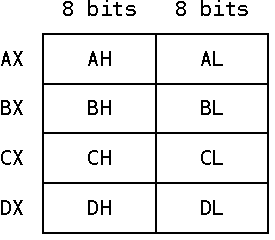
\includegraphics[width=.4\textwidth]{registers}
  \end{center}
  \caption{x86 registers}
  \label{fig:regs}
\end{figure}

\section{Interrupt Call}

BIOS interrupt calls perform hardware control or I/O functions requested by a program,
return system information to the program, or do both. A key element of the purpose of BIOS
calls is abstraction. The BIOS calls perform generally defined functions, and the specific
details of how those functions are executed on the particular hardware of the system are
encapsulated in the BIOS and hidden from the program\cite{wiki:bios-int}. The interrupt
calls are commonly used in RongOS are listed in Table~\ref{tbl:intcall}.

\begin{table}[!ht]
  \centering\tabulinesep=2mm
  \begin{tabu}{X[l,m,-1]X[l,m]X[-1,l,m]X[-1,l,m]}
    \tabucline-\rowfont\bfseries
    Interrupt\par{}Number & Register Parameter & Return Value & Function\\ \tabucline-
    0x10 &
    ah=0x0e(write character in tty mode)\par{}
    al=character code\par{}
    bh=0, bl=colorcolor& null & video services \\\tabucline-
    0x13 &
    ah=0x02(read sectors)\par{}
    ah=0x03(write sectors)\par{}
    ah=0x04(verify sectors)\par{}
    ah=0x0c(seek to specified track)\par{}
    al=number of sectors processing\par{}
    ch=cylinder \& 0xff  cl=sector number\par{}
    dh=header number dl=driver number\par{}
    es:bx=buffer address &
    FLACS.CF=0\par{}
    no error, ah = 0\par{}
    FLAGS.CF=1\par{}
    error, ah=error number\par{}& disk services \\ \tabucline-
  \end{tabu}
  \caption{RongOS interrupt calls}\label{tbl:intcall}
\end{table}

\section{Memory Map}

In the boot process, a memory map is passed on from the firmware in order to instruct an
operating system kernel about memory layout. It contains the information regarding the
size of total memory, any reserved regions and may also provide other details specific to
the
architecture\footnote{http://hypervsir.blogspot.com/2014/09/approach-to-retrieving-bios-memory-map.html}. For
loading RongOS to memory, the memory layout should be clarified as in
Table~\ref{tbl:memlayout}.


\begin{table}[!ht]
  \centering\tabulinesep=2mm
  \begin{tabu}{%
      >{\texttt\bgroup}r<{\egroup}@{\,--\,}>{\texttt\bgroup}l<{\egroup}%
      >{\texttt\bgroup}r<{\egroup}@{\,--\,}>{\texttt\bgroup}l<{\egroup}%
      >{\texttt\bgroup}l<{\egroup}l}%
    \tabucline-\rowfont\bfseries%
    \multicolumn{2}{l}{Range (in hexadecimal)} &%
    \multicolumn{2}{l}{Range (in decimal)} &%
    \multicolumn{1}{l}{Size (in bytes)} & Usage \\ \tabucline-
    0000 & 03ff & 0000 & 1023 & 1024 &  interrupt vector table \\ 
    0400 & 04ff & 1024 & 1279 & 256 & BIOS data area \\ 
    0500 & 051f & 1280 & 1311 & 32 & Reserved \\ 
    0520 & 7bff & 1312 & 31743 & 30432 & conventional memory \\ 
    7c00 & 7dff & 31744 & 32255 & 512 & master boot record \\ 
    7e00 & 9ffff & 32256 & 655359 & 623104 & conventional memory \\ 
    a0000 & affff & 655360 & 720895 & 64K & VGA graphics RAM \\ 
    b0000 & b7fff & 720896 & 753663 & 32K & monochrome text mode \\ 
    b8000 & bffff & 753664 & 786431 & 32K & color text mode \\ 
    c0000 & c7fff & 786432 & 819199 & 32K & VGA video ROM \\ 
    c8000 & cbfff & 819200 & 835583 & 16K & IDE hard drive \\ 
    cc000 & cffff & 835584 & 851967 & 16K & optional adapter \\ \tabucline-
  \end{tabu}
  \caption{RongOS Memory Layout}\label{tbl:memlayout}
\end{table}

\section{Floppy Disk}

There are many ways to boot an operating system, from hard disk, USB, floppy disk, etc.
The structure of floppy disk is simple and for this simple operating system it's enough.

Fig.~\ref{fig:flpy1.png} shows the inside of a floppy disk:
\begin{figure}[!ht]
  \centering
  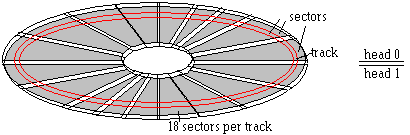
\includegraphics[width=.5\textwidth]{../figs/bootLoader/flpy1.png}
  \caption{Floppy disk structure}
  \label{fig:flpy1.png}
\end{figure}

A floppy disk, also called a floppy, diskette, or just disk, is a type of disk storage
composed of a disk of thin and flexible magnetic storage medium, sealed in a rectangular
plastic enclosure lined with fabric that removes dust particles. Floppy disks are read and
written by a floppy disk drive (FDD)\cite{wiki:floppy}.

For 3.5 inch HD floppy,  There are 80 cylinders from the outermost to
the core on each side, numbering 0, 1, \ldots, 79. The head can assign be 0 or 1,
representing two sides of floppy. When specify head number and cylinder number, forming a
ring, named track in jargon. The track is large so we divide it to 18 small parts, named
sector. A sector can store 512 byte. So the capacity of a floppy is:

\[18 \times 80 \times 2 \times 512 = 1474560\,Byte = 1440\,KiB\]

\fi


\chapter{Design}
In this section will introduce the design of the entire system including the kernel, API,
and applications.


\section{Top Level Design}
All applications use the functions provided by the operating system kernel through API
calls. This facilitates the application's ability to call the operating system. The
overall system architecture is as ~\ref{fig:top-level} shown:

\begin{figure}[!htbp]
  \centering
  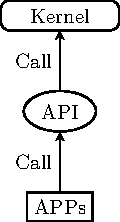
\includegraphics[width=0.5\textwidth]{topDes.pdf}
  \caption{Top-level design}
  \label{fig:top-level}
\end{figure}


\section{Detailed Design}
\label{sec:detailed-design}



\subsection{Kernel}
\label{sec:kernel}
The kernel receives the API call in the upward direction and the kernel requests the
hardware service through the driver in the downward direction.

\subsubsection{1. Module Relationship}
\label{sec:overview-1}

Fig. ~\ref{fig:kernel} shows how the various modules in
the kernel are related. \texttt{bootpack} completes startup-related settings such as
keyboard, PIC, GDT/IDT and mouse settings. \texttt{ipl} loads the entire operating system
into memory. \texttt{asmhead} completes the switch to 32-bit mode and calls the C
function. \texttt{naskfunc} is used to provide functions that the C language cannot do and
thus requires assembly. \texttt{PIC}, \texttt{keyboard} and \texttt{mouse} is used to
complete hardware-related initialization. \texttt{console} is used to accept command line
arguments and run various commands related to the application. \texttt{graphic} is used to
depict the mouse, graphics etc. \texttt{window} for making windows. \texttt{sheet} is used to
control layers, such as layer height settings etc. \texttt{memory} for managing
memory. \texttt{task} is used to manage multiple tasks, such as task switching,
scheduling. \texttt{timer} for managing time slices. \texttt{fifo} is used to manage FIFO buffers
that are used to accept various data. \texttt{dsctbl} for GDT/IDT setting. \texttt{file} is used to
manage file-related operations such as reading, loading, and searching for files. 


\begin{figure}[!htbp]
  \centering
  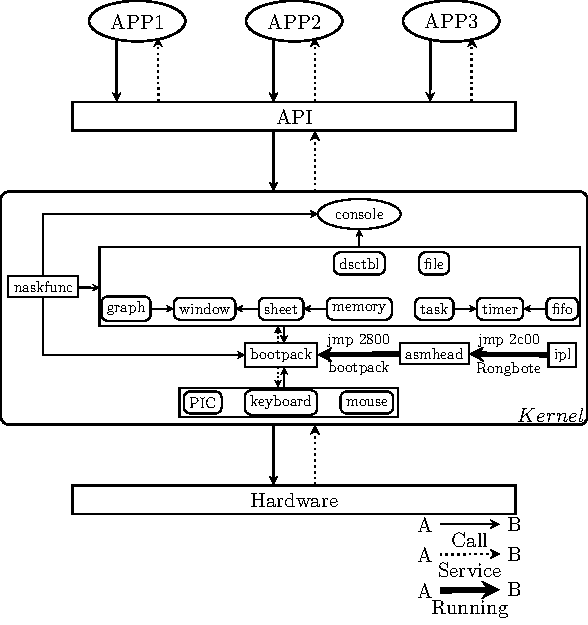
\includegraphics[width=0.9\textwidth]{topDesKernel}
  \caption{modules in kernel}
  \label{fig:kernel}
\end{figure}


\subsubsection{2. Data Structure in Kernel}
The following describes the data structure used in the RongOS operating system.

\label{sec:datastructure-kernel}
\begin{enumerate}
\item
  NAME \\
  \hspace*{1cm}\texttt{BOOTINFO} \\
  SYNOPSIS \\
  \hspace*{1cm}The structure \texttt{BOOTINFO} stores startup-related information, such as
  how many cylinders were read, the status of the keyboard indicator, the mode of the
  screen, the size of the screen, and the memory address of the graphics card. \\
  MEMBER \\
  \hspace*{1cm}char cyls \\
  \hspace*{1.5cm} number of cylinders to read \\
  \hspace*{1cm}char leds \\
  \hspace*{1.5cm} keyboard state at boot \\
  \hspace*{1cm}char vmode \\
  \hspace*{1.5cm} bits of color of graphics card \\
  \hspace*{1cm}char reserve \\
  \hspace*{1.5cm} reserved bytes \\
  \hspace*{1cm}short scrnx \\
  \hspace*{1.5cm} screen resolution of x \\
  \hspace*{1cm}short scrny \\
  \hspace*{1.5cm} screen resolution of y \\
  \hspace*{1cm}char* vram \\
  \hspace*{1.5cm}the starting address of the image buffer\\

  \item
  NAME \\
  \hspace*{1cm}\texttt{FIFO32} \\
  SYNOPSIS \\
  \hspace*{1cm} \texttt{FIFO32} is used to describe a FIFO structure. This
structure is used to receive various kinds of information. \texttt{FIFO32} is used to
describe a FIFO structure. This structure is used to receive various kinds of
information. It specifies where to read and write the FIFO structure and the size of the
buffer, available size.\\
  MEMBER \\
  \hspace*{1cm} int* buf \\
  \hspace*{1.5cm}  the address of FIFO32 buffer \\
  \hspace*{1cm} int p \\
  \hspace*{1.5cm} the writing address \\
  \hspace*{1cm} int q\\
  \hspace*{1.5cm} the reading address \\
  \hspace*{1cm} int size\\
  \hspace*{1.5cm} the size of FIFO32 buffer \\
  \hspace*{1cm} int free \\
  \hspace*{1.5cm} how many space free\\
  \hspace*{1cm} int flags\\
  \hspace*{1.5cm}  the states of FIFO32 buffer\\
  \hspace*{1cm} struct TASK* task \\
  \hspace*{1.5cm} point to a task \\

  \item
  NAME \\
  \hspace*{1cm}\texttt{SEGMENT\_DESCRIPTOR} \\
  SYNOPSIS \\
  \hspace*{1cm} \texttt{SEGMENT\_DESCRIPTOR} structure is
used to store GDT related information, which is based on CPU specifications(3.5.1 and
3.4.5\cite{intel_3a}). GDT is stored at 270000 in memory. \\
  MEMBER \\
  \hspace*{1cm} short limit\_low\\
  \hspace*{1.5cm}  the low part of segment size\\ 
  \hspace*{1cm} short base\_low\\
  \hspace*{1.5cm} the low part of base address\\
  \hspace*{1cm} char base\_mid\\
  \hspace*{1.5cm} the middle part of base address\\
  \hspace*{1cm} char access\_right\\
  \hspace*{1.5cm} read and write permissions etc\\
  \hspace*{1cm} char  limit\_high\\
  \hspace*{1.5cm} the high part of segment size\\
  \hspace*{1cm} char base\_high\\
  \hspace*{1.5cm}  the high part of base address\\

  \item
  NAME \\
  \hspace*{1cm}\texttt{GATE\_DESCRIPTOR} \\
  SYNOPSIS \\
  \hspace*{1cm} \texttt{GATE\_DESCRIPTOR} structure is used to
store IDT related information, which is based on CPU specifications(3.5.1 and
3.4.5\cite{intel_3a}). IDT is at 26f800 memory.\\
  MEMBER \\
  \hspace*{1cm} short offset\_low\\
  \hspace*{1.5cm}  the low part of offset\\
  \hspace*{1cm} short selector\\
  \hspace*{1.5cm} which interrupt to choose\\
  \hspace*{1cm} char dw\_count\\
  \hspace*{1.5cm} how many interrupts are registered\\
  \hspace*{1cm} char access\_right\\
  \hspace*{1.5cm} access permission\\
  \hspace*{1cm} short  offset\_high\\
  \hspace*{1.5cm} high part of offset\\

  \item
  NAME \\
  \hspace*{1cm}\texttt{MOUSE\_DEC} \\
  SYNOPSIS \\
  \hspace*{1cm} \texttt{MOUSE\_DEC} structure is used to store
information about the mouse, such as the location of the mouse, whether the mouse is
pressed or not.\\
  MEMBER \\
  \hspace*{1cm} unsigned char buf[3]\\
  \hspace*{1.5cm}  store the data from mouse\\
  \hspace*{1cm} unsigned char phase\\
  \hspace*{1.5cm} the stage of receiving mouse data\\
  \hspace*{1cm} int x\\
  \hspace*{1.5cm} the x point of mouse\\
  \hspace*{1cm} int y\\
  \hspace*{1.5cm} the y point of mouse\\
  \hspace*{1cm} int btn\\
  \hspace*{1.5cm} whether the mouse is pressed\\

  \item
  NAME \\
  \hspace*{1cm}\texttt{FREEINFO} \\
  SYNOPSIS \\
  \hspace*{1cm} \texttt{FREEINFO} structure stores how many bytes are
free from where in memory.\\
  MEMBER \\
  \hspace*{1cm} unsigned int addr\\
  \hspace*{1.5cm}  the starting address of free space\\
  \hspace*{1cm} unsigned int size\\
  \hspace*{1.5cm} how many size is free\\

  \item
  NAME \\
  \hspace*{1cm}\texttt{MEMMAN} \\
  SYNOPSIS \\
  \hspace*{1cm} \texttt{MEMMAN} structure is used to store the entire
memory usage, such as the total remaining memory space and entries.\\
  MEMBER \\
  \hspace*{1cm} int frees\\
  \hspace*{1.5cm}  how many memory blocks are free\\
  \hspace*{1cm} int maxfrees\\
  \hspace*{1.5cm} the maximum of frees\\
  \hspace*{1cm} int lostsize\\
  \hspace*{1.5cm} release the sum of the failed memory size\\
  \hspace*{1cm} int losts\\
  \hspace*{1.5cm}  the number of failures\\
  \hspace*{1cm} struct FREEINFO free[MEMMAN\_FREES]\\
  \hspace*{1.5cm} record all free memory block information\\

  \item
  NAME \\
  \hspace*{1cm}\texttt{SHEET} \\
  SYNOPSIS \\
  \hspace*{1cm}  \texttt{SHEET} structure is used to record the position,
usage, and color of a layer.\\
  MEMBER \\
  \hspace*{1cm} char* buf\\
  \hspace*{1.5cm}  the address of the graphic content depicted\\
  \hspace*{1cm} int bxszie\\
  \hspace*{1.5cm} the size of x coordinate of sheet\\
  \hspace*{1cm} int bysize\\
  \hspace*{1.5cm} the size of y coordinate of sheet\\
  \hspace*{1cm} int vx0\\
  \hspace*{1.5cm} the x coordinate of sheet\\
  \hspace*{1cm} int vy0\\
  \hspace*{1.5cm} the y coordinate of sheet\\
  \hspace*{1cm} int col\_inv\\
  \hspace*{1.5cm}  the number of invisible color\\
  \hspace*{1cm} int height\\
  \hspace*{1.5cm}  the height of sheet\\
  \hspace*{1cm} int flags\\
  \hspace*{1.5cm}  the states of sheet, using or not \\
  
  \item
  NAME \\
  \hspace*{1cm}\texttt{SHTCTL} \\
  SYNOPSIS \\
  \hspace*{1cm} \texttt{SHTCTL} structure is used to manage the structure
of multiple layer information, including how many layers there are in total, the size and
height of each layer.\\
  MEMBER \\
  \hspace*{1cm} unsigned char* vram\\
  \hspace*{1.5cm}  the address of VRAM\\
  \hspace*{1cm} unsigned char* map\\
  \hspace*{1.5cm} which layer the pixel on the screen belongs to\\
  \hspace*{1cm} int xsize \\
  \hspace*{1.5cm} the x size of screen\\
  \hspace*{1cm} int ysize\\
  \hspace*{1.5cm} the y size of screen\\
  \hspace*{1cm} int top\\
  \hspace*{1.5cm}  the height of the top layer\\
  \hspace*{1cm} struct SHEET* sheets[MAX\_SHEETS]\\
  \hspace*{1.5cm}  order all layer addresses in order\\
  \hspace*{1cm} struct SHEET sheets0[MAX\_SHEETS]\\
  \hspace*{1.5cm} all layers\\

  \item
  NAME \\
  \hspace*{1cm}\texttt{TIMER} \\
  SYNOPSIS \\
  \hspace*{1cm} \texttt{TIMER} structure is used to manage the time
slice of the CPU. The timer interrupts the CPU at regular intervals. This structure
records the length of the timer, usage status and other information.\\
  MEMBER \\
  \hspace*{1cm} struct TIMER* next\\
  \hspace*{1.5cm}  the next timer that is about to timeout\\
  \hspace*{1cm} unsigned int timeout\\
  \hspace*{1.5cm} how long is the timeout\\
  \hspace*{1cm} char flags\\
  \hspace*{1.5cm} the states of timer\\
  \hspace*{1cm} char flgas2\\
  \hspace*{1.5cm} whether to allow automatic cancellation\\
  \hspace*{1cm} struct FIFO32* fifo\\
  \hspace*{1.5cm} store data(from mouse, keyboard etc)\\
  \hspace*{1cm} int data\\
  \hspace*{1.5cm}  accept data\\

  \item
  NAME \\
  \hspace*{1cm}\texttt{TIMERCTL} \\
  SYNOPSIS \\
  \hspace*{1cm} \texttt{TIMERCTL} structure is used to manage all
timers in the system. Including how many timers are in total, current use, and the next
timer to be used.\\
  MEMBER \\
  \hspace*{1cm} unsigned int count\\
  \hspace*{1.5cm}  count variable\\
  \hspace*{1cm} unsigned int next\\
  \hspace*{1.5cm} the next timeout timer\\
  \hspace*{1cm} sturct TIMER* t0\\
  \hspace*{1.5cm} the shortest timeout timer\\
  \hspace*{1cm} struct TIMER timers0\\
  \hspace*{1.5cm} all timers\\

\item
  NAME \\
  \hspace*{1cm}\texttt{TSS32} \\
  SYNOPSIS \\
  \hspace*{1cm}  \texttt{TSS32} structure holds information about task
status segments, which are based on CPU specifications(See 6.2.1\cite{intel_3a}).\\
  MEMBER \\
  \hspace*{1cm} int esp0, esp1, esp2\\
  \hspace*{1.5cm}  stack pointer register\\
  \hspace*{1cm} int ss0, ss1, ss2\\
  \hspace*{1.5cm} stack segment register\\
  \hspace*{1cm} int cr3\\
  \hspace*{1.5cm} control register\\
  \hspace*{1cm} int eip\\
  \hspace*{1.5cm} instruct pointer register\\
  \hspace*{1cm} int eflags\\
  \hspace*{1.5cm} registers flag\\
  \hspace*{1cm} int eax\\
  \hspace*{1.5cm}  accumulator register\\
  \hspace*{1cm} int ecx\\
  \hspace*{1.5cm} counter register\\
  \hspace*{1cm} int edx\\
  \hspace*{1.5cm} data register\\
  \hspace*{1cm} int ebx\\
  \hspace*{1.5cm} base register\\
  \hspace*{1cm} int esp\\
  \hspace*{1.5cm}  stack pointer register\\
  \hspace*{1cm} int ebp\\
  \hspace*{1.5cm}  base pointer register\\
  \hspace*{1cm} int esi\\
  \hspace*{1.5cm} source index register\\
  \hspace*{1cm} int edi\\
  \hspace*{1.5cm}destination index register \\
  \hspace*{1cm} int es\\
  \hspace*{1.5cm}  extra segment register\\
  \hspace*{1cm} int cs\\
  \hspace*{1.5cm} code segment register\\
  \hspace*{1cm} int ss\\
  \hspace*{1.5cm} stack segment register\\
  \hspace*{1cm} int ds\\
  \hspace*{1.5cm} data segment register\\
  \hspace*{1cm} int fs\\
  \hspace*{1.5cm}  segment part 2\\
  \hspace*{1cm} int gs\\
  \hspace*{1.5cm} segment part 3\\
  \hspace*{1cm} int ldtr\\
  \hspace*{1.5cm}  LDT segment selector\\
  \hspace*{1cm} int iomap\\
  \hspace*{1.5cm} I/O map base address\\

\item
  NAME \\
  \hspace*{1cm}\texttt{FILEHANDLE} \\
  SYNOPSIS \\
  \hspace*{1cm} \texttt{FILEHANDLE} is used to record an open file related data structure\\
  MEMBER \\
  \hspace*{1cm} char* buf\\
  \hspace*{1.5cm}  store the handler of file\\
  \hspace*{1cm} int size\\
  \hspace*{1.5cm} the size of file\\
  \hspace*{1cm} int pos\\
  \hspace*{1.5cm} where to read the file\\

  \item
  NAME \\
  \hspace*{1cm}\texttt{TASK} \\
  SYNOPSIS \\
  \hspace*{1cm} \texttt{TASK} is used to manage variables for a task. Record the task's sections, permissions, stacks, etc.\\
  MEMBER \\
  \hspace*{1cm} int sel\\
  \hspace*{1.5cm}   the number of GDT\\
  \hspace*{1cm} int flags\\
  \hspace*{1.5cm} the state of task\\
  \hspace*{1cm} int level\\
  \hspace*{1.5cm} the level of task\\
  \hspace*{1cm} int priority\\
  \hspace*{1.5cm} the priority of task\\
  \hspace*{1cm} struct FIFO32 fifo\\
  \hspace*{1.5cm} a fifo buffer\\
  \hspace*{1cm} TSS32 tss\\
  \hspace*{1.5cm}  TSS segment for a task\\
  \hspace*{1cm} struct CONSOLE* cons\\
  \hspace*{1.5cm} the console window address of task\\
  \hspace*{1cm} int ds\_base\\
  \hspace*{1.5cm}  data segment address of APPs\\
  \hspace*{1cm} int cons\_stack\\
  \hspace*{1.5cm}  the stack address of APPs\\
  \hspace*{1cm} struct SEGMENT\_DESCRIPTOR ldt[2]\\
  \hspace*{1.5cm}  tow LDT segments of task\\
  \hspace*{1cm}  struct FILEHANDLE* fhandle\\
  \hspace*{1.5cm}  file handles for manipulating files \\
  \hspace*{1cm} int* fat\\
  \hspace*{1.5cm}  file allocation table\\
  \hspace*{1cm} char* cmdline\\
  \hspace*{1.5cm}  store the command line context\\
  \hspace*{1cm} unsigned char langmode\\
  \hspace*{1.5cm}  which font to use\\
  \hspace*{1cm} unsigned char langbyte1\\
  \hspace*{1.5cm}  store the first byte of the full-width character\\

  \item
  NAME \\
  \hspace*{1cm}\texttt{TASKLEVEL} \\
  SYNOPSIS \\
  \hspace*{1cm} \texttt{TASKLEVEL} is used to record information for all tasks on a layer\\
  MEMBER \\
  \hspace*{1cm} int running\\
  \hspace*{1.5cm}  how many tasks are running\\
  \hspace*{1cm} int now\\
  \hspace*{1.5cm} which task is currently running\\
  \hspace*{1cm} struct TASK* tasks[MAX\_TASKS\_LV]\\
  \hspace*{1.5cm} all tasks in one level\\

  \item
  NAME \\
  \hspace*{1cm}\texttt{TASKCTL} \\
  SYNOPSIS \\
  \hspace*{1cm} \texttt{TASKCTL} is used for all levels of tasks in the entire system.\\
  MEMBER \\
  \hspace*{1cm} int now\_lv\\
  \hspace*{1.5cm}  current activity level\\
  \hspace*{1cm} int lv\_change\\
  \hspace*{1.5cm} does the hierarchy need to be changed next time the task is switched\\

  \item
  NAME \\
  \hspace*{1cm}\texttt{CONSOLE} \\
  SYNOPSIS \\
  \hspace*{1cm} \texttt{CONSOLE} controls terminal window-related variables\\
  MEMBER \\
  \hspace*{1cm} struct SHEET* sht\\
  \hspace*{1.5cm}  which layer is used on the command line\\
  \hspace*{1cm} int cur\_x\\
  \hspace*{1.5cm} the x position of console\\
  \hspace*{1cm} int cur\_y \\
  \hspace*{1.5cm} the y position of console\\
  \hspace*{1cm} int cur\_c\\
  \hspace*{1.5cm} the color of console \\
  \hspace*{1cm} struct TIMER* timer\\
  \hspace*{1.5cm} timer to control cursor blinking\\
  
\item
  NAME \\
  \hspace*{1cm}\texttt{FILEINFO} \\
  SYNOPSIS \\
  \hspace*{1cm} \texttt{FILEINFO} is used to record file-related information, such as file name, size, etc.\\
  MEMBER \\
  \hspace*{1cm} unsigned char name[8]\\
  \hspace*{1.5cm}  file name\\
  \hspace*{1cm} unsigned char ext[3]\\
  \hspace*{1.5cm} extend name of file\\
  \hspace*{1cm} unsigned char type\\
  \hspace*{1.5cm}  file attributes\\
  \hspace*{1cm} char reserve[10]\\
  \hspace*{1.5cm} reserve byte\\
  \hspace*{1cm}  unsigned short time\\
  \hspace*{1.5cm} the time for storing file\\
  \hspace*{1cm} unsigned short date\\
  \hspace*{1.5cm}  the date for storing file\\
  \hspace*{1cm} unsigned short  clustno\\
  \hspace*{1.5cm}the file from which sector on the disk is stored \\


\end{enumerate}
    
\subsubsection{3. Each Module}
\label{sec:3.-modules-kernel}

\begin{enumerate}
\item
  \begin{itemize}
  \item NAME
    \begin{itemize}
    \item \texttt{graphic}
    \end{itemize}
    
  \item SYNOPSIS
    \begin{itemize}
    \item \texttt{graphic} is used to depict the mouse, graphics. Finish the palette setting etc.
    \end{itemize}
    
  \item FUNCTION
    \begin{itemize}
    \item \texttt{void init\_palette(void)}
      \begin{itemize}
      \item Objective: prepare the color definition and call the palette setting function
        \texttt{set\_palete()}.
      \item Parameter: NULL
      \end{itemize}
      
    \item \texttt{void set\_palette(int start, int end, unsigned char *rgb)}
      \begin{itemize}
      \item Objective: using the color variables prepared in the \texttt{init\_palette},
        the palette is set by calling the assembly function in \texttt{naskfunc} module to
        operate the hardware.
      \item Parameter
        \begin{itemize}
        \item \texttt{int start}: start color number
        \item \texttt{int end}: end color number
        \item \texttt{unsigned char* rgb}: the address of color buffer
        \end{itemize}
      \end{itemize}

    \item \texttt{}
      \begin{itemize}
      \item Objective:
      \item Parameter:
        \begin{itemize}
        \item
        \item
        \item
        \item
        \end{itemize}
      \end{itemize}
      
    \end{itemize}
    
  \end{itemize}


\item
  \begin{itemize}
  \item NAME
    \begin{itemize}
    \item \texttt{}
    \end{itemize}
    
  \item SYNOPSIS
    \begin{itemize}
    \item \texttt{}
    \end{itemize}
    
  \item FUNCTION
    \begin{itemize}
    \item \texttt{}
      \begin{itemize}
      \item Objective: 
        \texttt{}
      \item Parameter: 
      \end{itemize}
      
    \item \texttt{}
      \begin{itemize}
      \item Objective:
      \item Parameter
        \begin{itemize}
        \item \texttt{}
        \item
        \item
        \item
        \end{itemize}
      \end{itemize}

    \item \texttt{}
      \begin{itemize}
      \item Objective:
      \item Parameter:
        \begin{itemize}
        \item
        \item
        \item
        \item
        \end{itemize}
      \end{itemize}
      \end{itemize}
    
  \end{itemize}
  
  
\end{enumerate}

\subsection{API}
\label{sec:api}

\subsection{APPs}
\label{sec:apps-1}



\chapter{Implementation}

\section{Kernel}
\subsection{Boot Loader(ipl.asm)}

The boot loader is implemented in Intel assembly. It works as following:

\begin{enumerate}
\item \textbf{Display boot information:} Firstly, the code in boot sector (See
  Appendix~\ref{sec:dis-boo-inf}) outputs some boot information. When \texttt{al=0}, the
  null character of boot information hit. Interrupt \texttt{0x10} is used for showing a
  character.
\item \textbf{Read the second sector:} Then jump to load C0-H0-S2, \texttt{ax} register
  saved the address where beginning puts the sectors from floppy. And preparing parameters
  for interrupt \texttt{0x13} in registers. The \texttt{0x13} interrupt used for read
  sector from floppy to memory. (See Appendix~\ref{sec:rea-sec-sec}).
\item \textbf{Read two sides of a track:}
  
  If there is a carry indicating some thing went wrong while reading the floppy disk,
  reset the registers and try reading it again. The read process aborts after five
  unsuccessful read.

  Register \texttt{si} is a counter. If no carry (success), jump to next segment, as one
  sector has been read into memory already. The address should increase 512 byte. Then
  sector number (\texttt{cl} register) is added by 1 and compare it to 18, if it's smaller
  than 18, jump to \texttt{readloop}, read the next sector.

  If the value of \texttt{cl} register bigger or equal to than 18, meaning that one track
  18 sector in this side of floppy read already, then reversed the head, add 1 to
  \texttt{dh} register.

  If the value of \texttt{dh} register after adding larger than or equal to 2, it's saying
  the original head is 1, one track of two sides read already. Otherwise the value of
  \texttt{dh} register smaller than 2, read this side indicating by \texttt{dh} register,
  jump to \texttt{readloop} segmentation. Appendix~\ref{sec:rea-two-sid} is the code to
  perform this function.

  There is a pseudo code about this process:
  \begin{figure}[!ht]
    \centering
    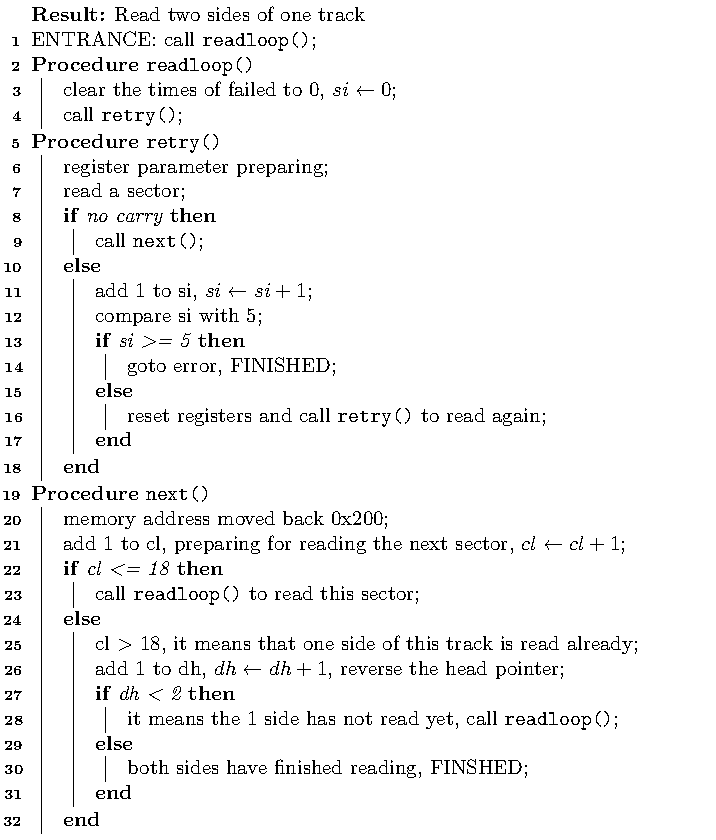
\includegraphics[width=.7\textwidth]{./figs/algorithm/read_two_side.pdf}
    \label{fig:read_two_sides}
  \end{figure}

  
  
\item \textbf{The next cylinder:} So the next step is moving a cylinder, add 1 to register
  \texttt{ch}. Otherwise the value of \texttt{dh} register smaller than 2, read this side
  indicating by \texttt{dh} register, jump to \texttt{readloop} segmentation. After
  \texttt{ch} register add 1, if it's smaller than 10, jump to \texttt{readloop},
  otherwise end loading floppy to memory process, for we only load ten cylinders of
  floppy. Appendix~\ref{sec:the-nex-cyl} is the code to perform this function.
\end{enumerate}

The above four steps can be intuitively reflected in the Fig. ~\ref{fig:iplflowchart}.
\begin{figure}[!htbp]
  \centering
  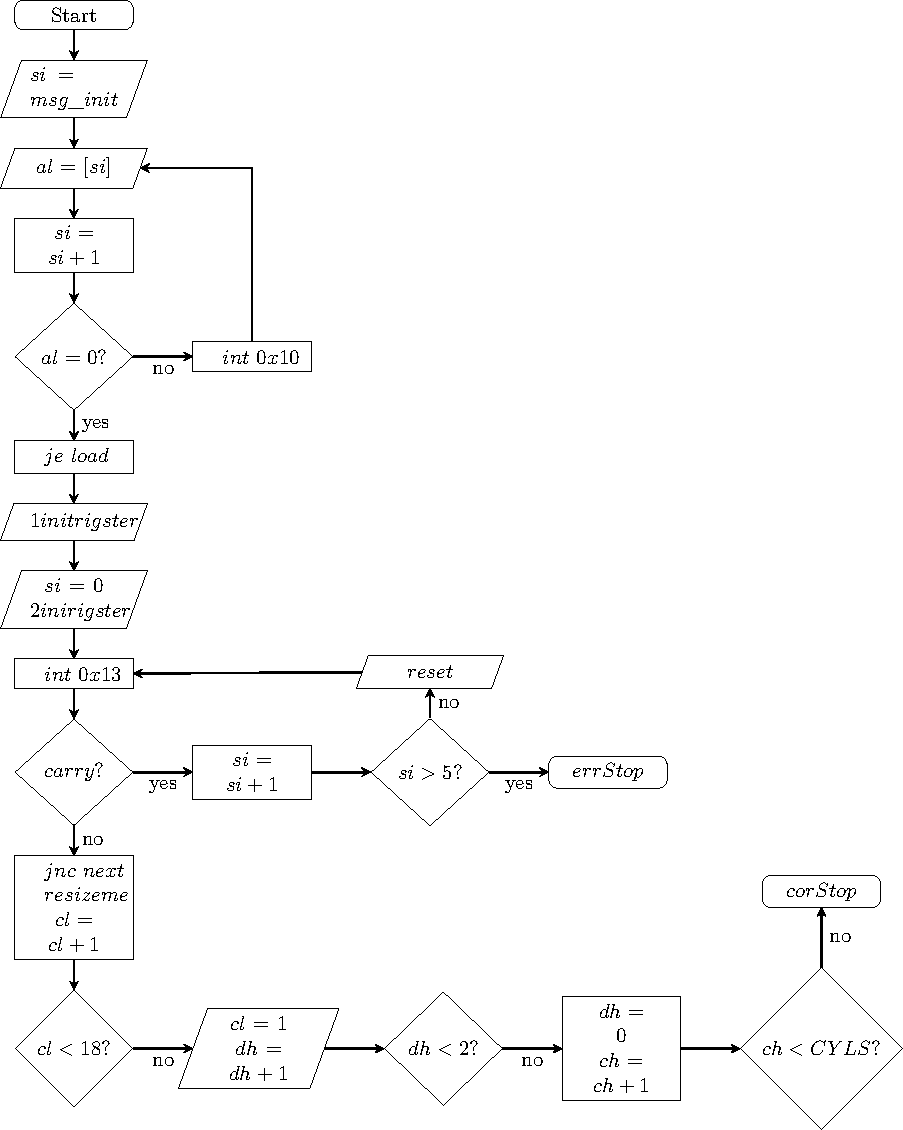
\includegraphics[width=1\textwidth]{flowchartp}
  \caption{the working flowchart of boot loader}
  \label{fig:iplflowchart}
\end{figure}

\section{API}
\label{sec:API}


\section{APPs}
\label{sec:apps}




\chapter{Conclusions}%{Prospects And Shortages}

\footnotetext{\url{https://thesistips.wordpress.com/2012/03/25/how-to-write-your-introduction-abstract-and-summary/}}

\paragraph{What goes in your ``Conclusions'' chapter?}

{\fontspec[Scale=.8]{Purisa} The purpose of this chapter is to provide a summary of the
  whole thesis or report.  In this context, it is similar to the Abstract, except that the
  Abstract puts roughly equal weight on all thesis/report chapters, whereas the
  Conclusions chapter focuses primarily on the findings, conclusions and/or
  recommendations of the project.

  There are a couple of rules – one rigid, one common sense, for this chapter:
  \begin{itemize}
  \item All material presented in this chapter must have appeared already in the report;
    no new material can be introduced in this chapter. (rigid rule of technical writing)
  \item Usually, you would not present any new figures or tables in this chapter. (rule of thumb)
  \end{itemize}

  Generally, for most technical reports and Masters theses, the Conclusions chapter would
  be~3 to 5 pages long (double spaced).  It would generally be longer in a large PhD
  thesis. Typically you would have a paragraph or two for each chapter or major
  subsection.  Aim to include the following (typical) content.
  \begin{enumerate}
  \item Re-introduce the project and the need for the work – though more briefly than in
    the intro;
  \item Re-iterate the purpose and specific objectives of your project.
  \item Re-cap the approach taken – similar to the road map in the intro; however, in this
    case, you are re-capping the data, methodology and results as you go.
  \item Summarize the major findings and recommendations of your work.
  \item Make recommendations for future research.
  \end{enumerate}}

%%% 正文部分到此结束。下面是『参考文献』、『指导教师简介』、『鸣谢』、『附录』

%% 不要动下面四行!
\appendix{}
\printbibliography[heading={bibintoc},title={Bibliography}] % 输出参考文献
\advisorinfopage{}                 % 输出指导教师简介
\acknowledgmentspage{}             % 输出鸣谢

%%% 下面是附录部分,可以没有。

\chapter{Main Program Code} %附录一

\section{Boot loader}

\subsection{Display boot information}
\label{sec:dis-boo-inf}

\inputminted[firstline=55, lastline=65,
linenos=true]{nasm}{../../src/kernel/ipl10.asm}

\subsection{Read the second sector}
\label{sec:rea-sec-sec}
  
\inputminted[firstline=87,lastline=106,linenos=true]{nasm}{../../src/kernel/ipl10.asm}

\subsection{Read two sides of a track}
\label{sec:rea-two-sid}

\inputminted[firstline=108,lastline=132,linenos=true]{nasm}{../../src/kernel/ipl10.asm}

\subsection{The next cylinder}
\label{sec:the-nex-cyl}

\inputminted[firstline=134,lastline=137,linenos=true]{nasm}{../../src/kernel/ipl10.asm}

\end{document} % 结束。不要动下面几行!

%%% Local Variables:
%%% mode: latex
%%% TeX-master: t
%%% End:
